
Estimating treatment effects of policy interventions in panel data is a challenging task due to the presence of unobserved counterfactuals and the need for robust estimation methods.
Traditional econometric methods have been widely used for their ability to model these counterfactuals and provide reliable estimates and confidence intervals under paticular assumptions, most closely based on the potential outcomes framework of \textcite{rubin1974estimating}.
However, these methods often implicitly or explicitly assume parametric forms of the data generating process, such as linearity or normality, which may not hold in practice.

This study explores the possibility of applying convolutional neural networks (CNNs) to panel data, particularly in the context of causal inference.
Multiple studies have used nontraditional methods 
or machine learning methods to estimate treatment effects in panel data.
For example, \textcite{athey2021matrix} have proposed a matrix completion method with nuclear norm regularization (MC-NNM henceforth) to estimate treatment effects in panel data that relies on cross validation to choose the
right degree of regularization.
Also, \textcite{abadie2010synthetic} have proposed a synthetic control method that uses 
a weighted average of control units to construct a counterfactual for the treated unit.
A natural extension to these methods is to use neural networks, which have shown remarkable performance in prediction tasks of high-dimensional data, such as images and text.


The main task of this study is to predict the counterfactual outcomes of a treated unit in a panel data setting with CNN, denoted 
as $\mathbf{Y(0)}$ in equation \eqref{eq:panel_data_Y0}.
Each row of $\mathbf{Y(0)}$ represents the sequence of outcomes of a unit, and the columns represent different time periods.
The treated unit is in the first row, and the red ${\color{red} ?}$'s are the missing counterfactuals we want to predict, as the treated unit's $Y(0)$'s are not observed after the treatment.
The other rows are the outcomes of control units, which are observed for all time periods.

\begin{align}
    	\mathbf{Y(0)}&=\begin{pmatrix}
		\tick  & \tick & {\color{red} ?}   & \dots & {\color{red} ?}  & \leftarrow{\text{treated unit}}\\
		\vdots   &  \vdots & \vdots &\ddots &\vdots& \\
        \tick & \tick & \tick  & \dots & \tick& \\
		\tick  & \tick & \tick   & \dots & \tick & \\
		\tick & \tick & \tick   & \dots & \tick & 
		\end{pmatrix} 
        \label{eq:panel_data_Y0}
\end{align}


\section{CNNs for Panel Data}


\subsection{Combining CNNs and Mahalanobis Distance}

Applying CNNs to panel data, however, is not as straightforward as applying them to images.
In images, the input is a 2D matrix of pixel values, and applying convolution operations are reasonable
because nearby pixels are likely to be correlated to each other.
In panel data, although the input is also a 2D matrix, the rows represent different units and the columns represent different time periods.
The correlation between different periods of the same unit is necessarily strong, but the correlation between adjacent units is not necessarily strong.
Put more simply, although the horizontal neighbors of each cell in $\mathbf{Y(0)}$ are likely to be correlated, the vertical neighbors are not.
Therefore, applying CNN to panel data requires modifying $\mathbf{Y(0)}$ so that vertically adjacent cells are also correlated.

To tackle the aforementioned issue, we propose a novel approach that combines CNNs and Mahalanobis covariate distance to estimate causal effects in panel data.
The Mahalanobis distance is a measure of the distance between a point and a distribution, which takes into account the covariance structure of the data:

\begin{align}
    d_{\text{Mahalanobis}}(\mathbf{x}, \mathbf{y}) &= \sqrt{(\mathbf{x} - \mathbf{y})^\top \Sigma^{-1} (\mathbf{x} - \mathbf{y})}  \qquad \text{where } \Sigma = \text{cov}(\mathbf{x}, \mathbf{y})\label{eq:mahalanobis_distance}
\end{align}

We compute \eqref{eq:mahalanobis_distance} between the treated unit and each control unit before the treatment, 
and use this Mahalanobis distance to order the control units vertically in $\mathbf{Y(0)}$.
This way, the vertically adjacent cells in $\mathbf{Y(0)}$ are more likely to be correlated, and applying CNNs to $\mathbf{Y(0)}$ is more reasonable:

\begin{align}
        \mathbf{Y(0)}&=\begin{pmatrix}
        \tick  & \tick & {\color{red} ?}   & \dots & {\color{red} ?}  &\\
        \vdots   &  \vdots & \vdots &\ddots &\vdots& \\
        \tick & \tick & \tick  & \dots & \tick& \\
        \tick  & \tick & \tick   & \dots & \tick & \\
        \tick & \tick & \tick   & \dots & \tick &
        \end{pmatrix} 
        \quad
        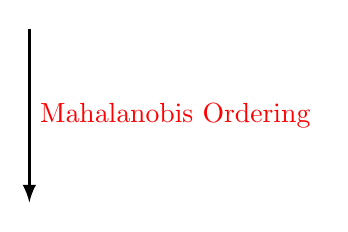
\begin{tikzpicture}[baseline={(current bounding box.center)}]
            \draw[very thick,->,>=latex] (0,1.2) -- (0,-1) node[midway,right] {\textcolor{red}{Mahalanobis Ordering}};
        \end{tikzpicture}
\end{align}


\subsection{CNN Configuration}
As opposed to images, the input of CNNs for panel data illustrated in \eqref{eq:panel_data_Y0} is a small matrix of outcomes, 
and thus a complex CNN architecture with too many parameters may lead to overfitting.
Thus, we use a simple CNN architecture with only two convolutional layers: the first layer has 32 filters of size 3$\times$3 with ReLU activation,
and the second layer has one filter of size 3$\times$3 with linear activation.
Both layers use a stride of 1 and zero padding to maintain the input size.
The output of the second layer is a $N \times T$ matrix, where $N$ is the number of units and $T$ is the number of time periods (i.e., the same size as $\mathbf{Y(0)}$).
The CNN is trained to minimize the mean squared error between the predicted outcomes and the actual outcomes of the control units ove all time periods,
and the optimization is performed using the Adam optimizer.